% \begin{SCfigure}[][htbp]
\begin{figure}[htp]

\begin{center}
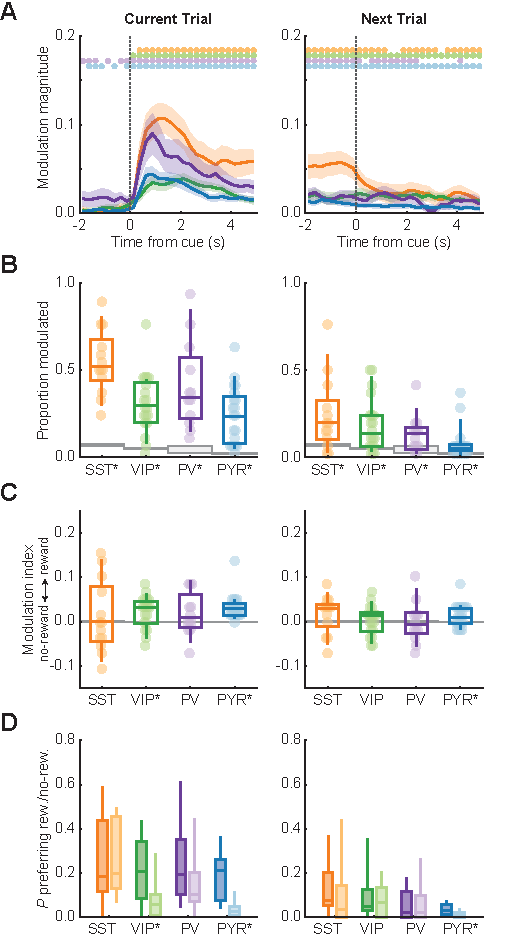
\includegraphics[width=8.7cm]{Figures/Chapter4/Fig7}
\end{center}

\caption[Outcome-related modulation]
{Outcome-related modulation. (A) Modulation magnitude $M$ with respect to the outcome of the current (left) and prior trial (right), plotted as in Figure \ref{fig:Fig6}A. Solid circles indicate time bins where $M_{\mathit{outcome}}(t)$ differed significantly from chance ($p<0.05$, Wilcoxon signed-rank test vs. shuffle) within SST (orange), VIP (green), PV (purple), and PYR populations (blue). (B) The proportion of each cell population, $P_{\mathit{outcome}}$, that exhibited significant modulation associated with the current (left) or prior outcome (right). (C) The mean modulation index $\bar{I}_{\mathit{outcome}}$ associated with the current (left) and prior outcome (right), calculated from the first 5 s of the trial. (D) The proportion of each cell population exhibiting a significant preference for rewarded ($P^+$; dark shading) and unrewarded choices ($P^-$; light shading), represented respectively in paired box plots. Left and right axes present the results with respect to the current and prior outcome, respectively. Asterisks in B--C indicate significant differences from the null distribution for each cell type; in D, they indicate significant differences between $P^+$ and $P^-$ within each cell type; both were assessed at $\alpha = 0.05$, Wilcoxon signed-rank test. $N=$ 13 SST, 19 VIP, 12 PV, and 20 PYR populations. All plots presented as in Figure \ref{fig:Fig6}.}

\label{fig:Fig7}
% \end{SCfigure}
\end{figure}

% {Outcome-related modulation. (A) Modulation magnitude $M$ with respect to the outcome of the current (left) and prior trial (right), plotted as a function of time relative to the sound cue. $M_{\mathit{outcome}}(t)$ is presented as the difference from a null distribution obtained when the same analysis was conducted using shuffled choices. Line plots with shaded confidence intervals represent the $\mathit{mean} \pm \mathit{SEM}$ within SST (orange), VIP (green), PV (purple), and PYR populations (blue). Solid circles above indicate time bins where $M_{\mathit{outcome}}(t)$ differed significantly from chance ($p<0.05$, Wilcoxon signed-rank test). (B) The proportion of each cell population, $P_{\mathit{outcome}}$, that exhibited significant modulation associated with the current (left) or prior outcome (right). (C) The mean modulation index $\bar{I}_{\mathit{outcome}}$ associated with the current (left) and prior outcome (right), calculated from the first 5 s of the trial. (D) The proportion of each cell population exhibiting a significant preference for rewarded ($P^+$) or unrewarded choices ($P^-$), represented respectively in paired box plots. Left and right axes present the results with respect to the current and prior outcome, respectively. Asterisks in B--C indicate significant differences from the null distribution for each cell type; in D, they indicate significant differences between $P^+$ and $P^-$ within each cell type; both were assessed at $\alpha = 0.05$, Wilcoxon signed-rank test. All plots presented as in Figure \ref{fig:Fig5}.}